\maketitle
\section{Introduction}

Considering a computer network an attacker would want to corrupt the computer with the
most power to either cause as much damage as possible, sniff as much data as possible or to
gain as much influence as possible. Naturally the owner of the network has the aim to protect
these most important targets especially well. The measure, of what the most important and 
powerful nodes in the network are, can be defined in different ways that fit different scenarios.
For instance if an attacker would want to sniff as much data as possible he would want to
attack the computer that forwards the highest amount of data between machines. However, an
attacker might also be targeting the nodes with the least power under the assumption that
those will have less protection and are easier to attack. This suggests that it might be
sensible to consider extra protection for the powerless nodes.

The following will provide a summary of popular centrality measures, how those can be used in
the context of penetration testing with a focus on the tool Bloodhound, documentation for the
provided centrality measurement tool and an example for the calculation of dependency
centrality visualizing the convergence of the Sinkhorn-Knopp method.

\section{Different Measures of Centrality}

The question of what node in a network is the most central one is often interesting
and important for making the optimal decision for many cases in multiple fields. 
The four most common centrality measures are degree-, closeness-, betweenness- and eigenvector 
centrality. The following describes those measures and will introduce an additional kind of 
centrality named dependency centrality. Networks are represented as graphs.

\paragraph{Degree Centrality}\mbox{} \medskip \\
The most central nodes are the ones that are connected to the most other nodes.
Which more precisely means the nodes for which the amount of edges that contain them is the highest. 
An application of this measure would be to ask what twitter account has the most followers.
Here twitter accounts are the nodes and the fact that one account follows another corresponds 
to an edge between those accounts/nodes.

\paragraph{Closeness Centrality}\mbox{} \medskip \\
The most central nodes are the ones that are on average the closest to every other node
in the graph with closeness meaning the minimum number of edges one has to travel to get to another node.

\paragraph{Betweenness Centrality}\mbox{} \medskip \\
For this measure, to find the most central node, one first considers every shortest
path between every node. The node that lies on the highest amount of such paths is the
most central one. An example where this measure would be interesting is in a network
of computers if an attacker wants to sniff as much traffic between those computers as possible.
The most ideal target would be the most central one according to betweenness centrality.

\paragraph{Eigenvector Centrality}\mbox{} \medskip \\
The most central node is recursively defined as the node that is connected to the highest number
of other nodes that themselves have a high degree of centrality again. In a network of Facebook
accounts, with the fact that one account is befriended with another as an edge, eigenvector centrality
would be a good measure to determine what account can influence the most users. For this problem it would
not fit to use degree centrality since the account that has the most friends does not necessarily
have the most reach. The account with the most influence is rather the one that has a lot of friends
that themselves have a lot of friends and so on.

\paragraph{Dependency Centrality}\mbox{} \medskip \\
The most central node is defined as the node that is connected to the most powerless nodes. This 
measure is interesting in situations where powerless actors are dependent on powerful actors, 
enabling the powerful nodes to threaten weaker ones to enforce their will.

\section{Calculating Centrality}

Since the way to calculate degree-, closeness- or betweenness centrality is already given by their 
definitions the focus in this section is on determining eigenvector- and dependency centrality.

\subsection{Eigenvector Centrality Calculation}
Graphs can be represented as adjacency matrices of size $n \times n$ with $n$ as the number of nodes.
Each node of the graph corresponds to a row and a column of the matrix. If there is an edge from node
$a$ to node $b$ in the graph, then in the matrix there is a one in row $a$ and column $b$.
\begin{table} [h]
    \begin{tabular} { cc }
        \parbox{5cm}{       
            \begin {tikzpicture}[-latex ,auto ,on grid ,
                    semithick, state/.style ={ circle ,top color =white, draw, minimum width =.5 cm}]
                \node[state] (a) {$a$};
                \node[state] (b) [below right = of a] {$b$};
                \node[state] (c) [below right = of b] {$c$};
                \node[state] (d) [below right = of c] {$d$};
                \node[state] (e) [below right = of d] {$e$};
                \path (a) edge [-] (b);
                \path (b) edge [-] (c);
                \path (c) edge [-] (d);
                \path (d) edge [-] (e);
            \end{tikzpicture}
        }
        \centering
        \parbox{5cm}{
            \begin{large}
                \[
                \begin{blockarray}{cccccc}
                    \mbox{} & a & b & c & d & e \\
                    \begin{block}{c(ccccc)}
                        a & 0 & 1 & 0 & 0 & 0   \\
                        b & 1 & 0 & 1 & 0 & 0   \\
                        c & 0 & 1 & 0 & 1 & 0   \\
                        d & 0 & 0 & 1 & 0 & 1   \\
                        e & 0 & 0 & 0 & 1 & 0   \\
                    \end{block}
                \end{blockarray}
                 \]
            \end{large}
        }
    \end{tabular}
    \captionsetup{type=figure}
    \caption{The corresponding adjacency matrix to a graph}
    \label{table:GraphToAdjacencyMatrix}
\end{table}
\mbox{} \\
For this adjacency matrix one can calculate the eigenvectors $x$ and the corresponding 
eigenvalues $ \lambda $ that solve the equation $Ax = \lambda x$. The important eigenvector is the one 
with the highest eigenvalue. In this vector the index of the highest entry is the 
index of the row and the column that corresponds to the most central node.



%TODO Vektoren und Eigenwerte als Visualisierung

\subsection{Dependency Centrality Calculation}

Calculating Dependency Centrality is in a sense the opposite of calculating Eigenvector Centrality.
Instead of finding the node that is connected to the most nodes that themselves are connected to many
nodes described in $Ax = \lambda x$, the goal is to find the node that is connected to the most other
nodes that themselves are connected to the least other nodes expressed in the equation $Ax^\div=x$
where $x^\div$ means the inverse of $x$ as described in the following. The goal is now to find a
vector $x$ that solves this equation.

\paragraph{Component wise Inverse of a Vector} \mbox{} \medskip \\
The component wise inverse of the vector $x$ written as $x^\div$ means the vector where each entry is the reciprocal
of the entry in the same row in $x$.

\paragraph{The Balancing Problem} \mbox{} \medskip \\
Given a matrix $A$ the balancing problem tries to find a matrix $D$ with a positive diagonal that
leads to $DAD=S$ being doubly stochastic. A matrix is double stochastic if the sum of each column
and the sum of each row is $1$. \\
Now about the connection between the balancing problem and dependency centrality.
Consider $D_{x^\div}$ as the diagonal matrix, with the entries of $x^\div$ on its main diagonal.
It turns out that $D_{x^\div}$ is a solution for the balancing problem for $A$ if and only if $x$
is a solution for $Ax^\div=x$ \parencite{2016-bozzo-a} which means that knowledge about solutions for 
the balancing problem can be used for the dependency centrality problem.

\paragraph{Term Rank} \mbox{} \medskip \\
The term rank of an adjacency matrix $A$ is defined as the maximum number of ones in $A$ with none of the
ones in the same column or row of $A$. However, for computing the term rank the Konig-Egervary Theorem
is used which states that the term rank of an adjacency matrix is equal to the minimum of the number 
of either rows or columns that contain all the ones of the matrix \parencite{1978-Brualdi-Matrices}.

\paragraph{Indecomposable, Total Support and Fully Indecomposable} \mbox{} \medskip \\
For calculating whether or not an adjacency matrix has total support, is indecomposable or is
fully indecomposable, the algorithms were chosen regarding efficiency instead of directly implementing
the terms definitions.\\

Let $A(i,j)$ be the adjacency matrix $A$ of size $n\times n$ without the row $i$ and
without the column $j$ and $t(A)$
the term rank of $A$. Then the matrix $A$ has total support if and only if $t(A(i,j))=n-1$
for every $i,j$ where $a_{i,j}=1$ with $a_{i,j}$ being the entry of $A$ in row $i$ and 
column $j$ \parencite{1978-Brualdi-Matrices}. This definition of total support is the one implemented
in the \texttt{Network Centrality Calculator}.\\
Regarding full indecomposability it is used that $A$ is fully indecomposable if and only if $t(A(i,j))=n-1$ 
for every $i,j$ \parencite{1978-Brualdi-Matrices}.
Lastly to calculate whether or not $A$ is indecomposable the strongly connected components algorithm of
Dijkstra is used to find out whether or not the graph of $A$ is a single strongly connected component.
If and only if that is the case $A$ is indecomposable \parencite{1976-dijkstra-a}.\\

These terms are important for the balancing problem, and therefore dependency centrality, since indecomposability
implies that the balancing problem has at leas one solution, total support implies at most one solution and
full indecomposability means that there is exactly one solution.


\paragraph{Guaranteeing that a solution exists} \mbox{} \medskip \\
Diagonal perturbation of the $n\times m$ adjacency matrix $A$ means the component wise addition of a
diagonal $n\times m$ matrix $D$, with only 
ones on its main diagonal, multiplied by a constant $\alpha$.

Meanwhile full perturbation means the component wise addition of a full matrix $F$, with ones as every
entry, multiplied by $\alpha$, to $A$.

These operations are helpful since they guarantee a solution for the balancing problem and therefore 
the problem of finding the most central node according to dependency centrality.
More precisely, diagonal perturbation leads to total support, implying at least one solution and
full perturbation leads to full indecomposability implying exactly one solution \parencite{2016-bozzo-a}.

It is clear that perturbation has an impact on the final result. How this is the case is visualized
in the example and convergence section.

\paragraph{The Sinkhorn-Knopp Method} \mbox{} \medskip \\
An easy approach to solving the balancing problem for $A$ and to finding the centralities according to dependency
centrality by solving $Ax^\div=x$, is the Sinkhorn-Knopp method. This method iteratively applies
$x_{k+1}=Ax_{k}^\div$ with a vector of ones as the starting vector.
If $A$ has total support the series of $x_{k}$ with an even $k$ and the series with an uneven $k$ will
converge, meaning that each entry of the vector converges. Hereby the uneven series and the even series
differ by a constant ratio. This is further highlighted in the example and convergence section.

\section{Tool: Network Centrality Calculator}

The Network Centrality Calculator provides the functionality to upload a graph as
a \texttt{.txt} or a \texttt{.csv} file. This file has to contain a list of edges written in the format
of firstly the name of a node, secondly a space or a comma and thirdly the name of the node the first one is connected to.
The next edge in the list is separated from the previous one by a new line.

\begin{table} [h]
    \begin{tabular} { cc }
        \parbox{5cm}{       
            \begin {tikzpicture}[-latex ,auto ,on grid ,
                    semithick, state/.style ={ circle ,top color =white, draw, minimum width =.5 cm}]
                \node[state] (a) {$a$};
                \node[state] (b) [below right = of a] {$b$};
                \node[state] (c) [above = of b] {$c$};
                \path (a) edge [-] (b);
                \path (b) edge [-] (c);
                \path (a) edge [-] (c);
            \end{tikzpicture}
        }
        \centering
        \parbox{5cm}{
            \texttt{a b\\
                b c\\
                c a\\
                b a\\
                c b\\
                a c
            }    
        }
    \end{tabular}
    \captionsetup{type=figure}
    \caption{The graph on the left can be uploaded as a .txt file with the content on the right}
    \label{table:GraphAsTxtFile}
\end{table}
\mbox{} \\
The uploaded graph will be displayed on the
right side of the page. The dropdown menu, with the default \texttt{degree centrality}, enables
the user to choose a centrality measure.
After a graph is uploaded the calculation of the centralities for the chosen measure begins. 
As soon as the results are available a table
appears with the names of the nodes in the first column their centralities in the second. The rows
are sorted by centralities while the node with the highest centrality is on top.
\begin{figure}[H]
    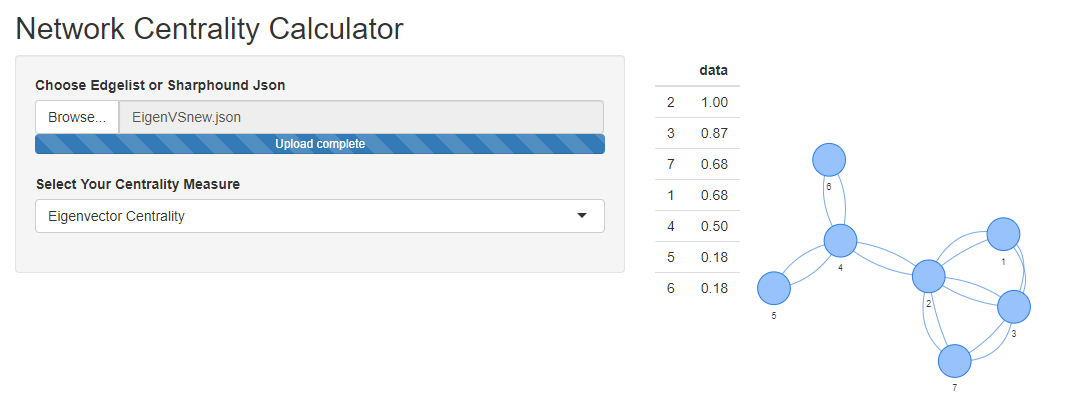
\includegraphics[width=\textwidth]{images/figures/calculatorEigenExample.PNG}        
    \caption{Screenshot of the tool with eigenvector centrality as selected measure}
\end{figure}
If the chosen centrality measure is \texttt{dependency centrality} several new inputs appear
and the user is informed whether the given graph is fully indecomposable, indecomposable or has 
total support and whether or not the Sinkhorn-Knopp method converges.
The first input is the number of Sinkhorn-Knopp steps that will be performed with a default
value of 100. The second input is a dropdown with the possibility to choose between no perturbation,
diagonal perturbation or full perturbation. With perturbation chosen the user also has the ability
to specify the $\alpha$ to multiply the perturbation matrix with as seen in the following figure.
\begin{figure}[ht]
    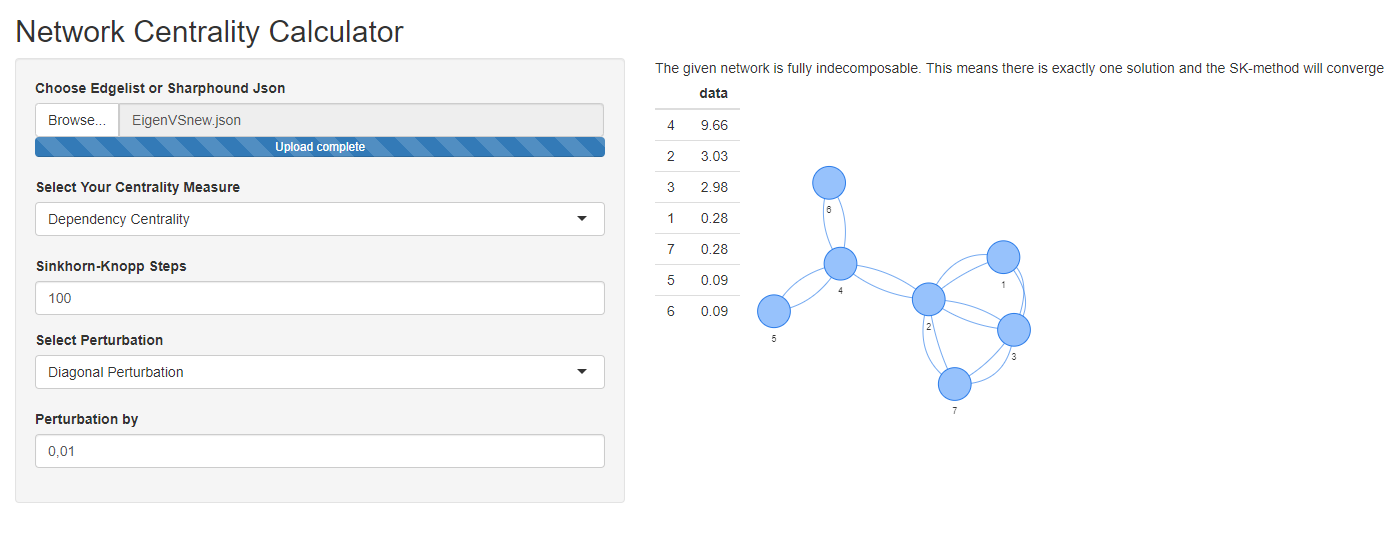
\includegraphics[width=\textwidth]{images/figures/calculatorDependencyExample.PNG}        
    \caption{Screenshot of the tool with all expanded options}
\end{figure}

\section{Bloodhound and Sharphound}

Bloodhound is a tool developed for discovering attack paths with the goal of getting access to
Computers, Users and Domain Controllers in an Active Directory context.
The Bloodhound ingestor called Sharphound can be used to fetch data from active directory networks.
This data with the underlying graph is saved to a \texttt{.json} file containing an array of 
nodes and an array of edges.
Each node has an attribute for the id, label, coordinates, type and more while 
the directed edges main attributes are a source node, a target node an id and a label.
Penetration testers can use this data to find out the most potent attack paths and take
measures to protect those. 

To analyze the network and to gain insight about the centrality of each node, a penetration
tester can use the provided \texttt{Network Centrality Calculator} which is abled to parse a 
\texttt{.json} file in the format that Sharphound produces. Instead of uploading a \texttt{.txt}
or \texttt{.csv} file, the Sharphound file can be uploaded, the graph will be extracted
and the centralities for the selected measure are calculated immediately after uploading.

\section{Example and convergence}

The following graph, called a kite network, is analyzed regarding its centralities with 
the network centrality calculator tool where dependency centrality is chosen as the measure.

\begin{figure}[ht]
    \centering
\begin {tikzpicture}[-latex ,auto ,on grid ,
                    semithick, state/.style ={ circle ,top color =white, draw, minimum width =.5 cm}]
                \node[state] (1) {$1$};
                \node[state] (2) [right = of 1] {$2$};
                \node[state] (3) [right = of 2] {$3$};
                \node[state] (4) [below right = of 3] {$4$};
                \node[state] (5) [above right = of 3] {$5$};
                \node[state] (6) [below right = of 4] {$6$};
                \node[state] (7) [below right = of 5] {$7$};
                \node[state] (8) [above right = of 5] {$8$};
                \node[state] (9) [below right = of 7] {$9$};
                \node[state] (10) [above right = of 7] {$10$};
                \path (1) edge [-] (2);
                \path (2) edge [-] (3);
                \path (3) edge [-] (4);
                \path (3) edge [-] (5);
                \path (5) edge [-] (8);
                \path (5) edge [-] (10);
                \path (5) edge [-] (7);
                \path (5) edge [-] (4);
                \path (4) edge [-] (7);
                \path (4) edge [-] (9);
                \path (4) edge [-] (6);
                \path (10) edge [-] (8);
                \path (10) edge [-] (7);
                \path (10) edge [-] (9);
                \path (9) edge [-] (7);
                \path (9) edge [-] (6);
\end{tikzpicture}
\caption{The kite network is indecomposable but has no total support. This means at most one solution exists
but it is not guaranteed that a solution exists.}
\end{figure}

To guarantee that a solution exists the adjacency matrix of the graph is diagonally perturbed with
$\alpha =0.0001$. After this the matrix is fully indecomposable and the Sinkhorn-Knopp method will
converge. With 100 steps of the Sinkhorn-Knopp method node $2$ turns out to be the most central one.
The unintuitive component wise convergence of the even and odd iteratives becomes clearer when visualized. 

\begin{figure}[H]
    \centering
    \begin{subfigure}[b]{.45\textwidth}
        \centering
        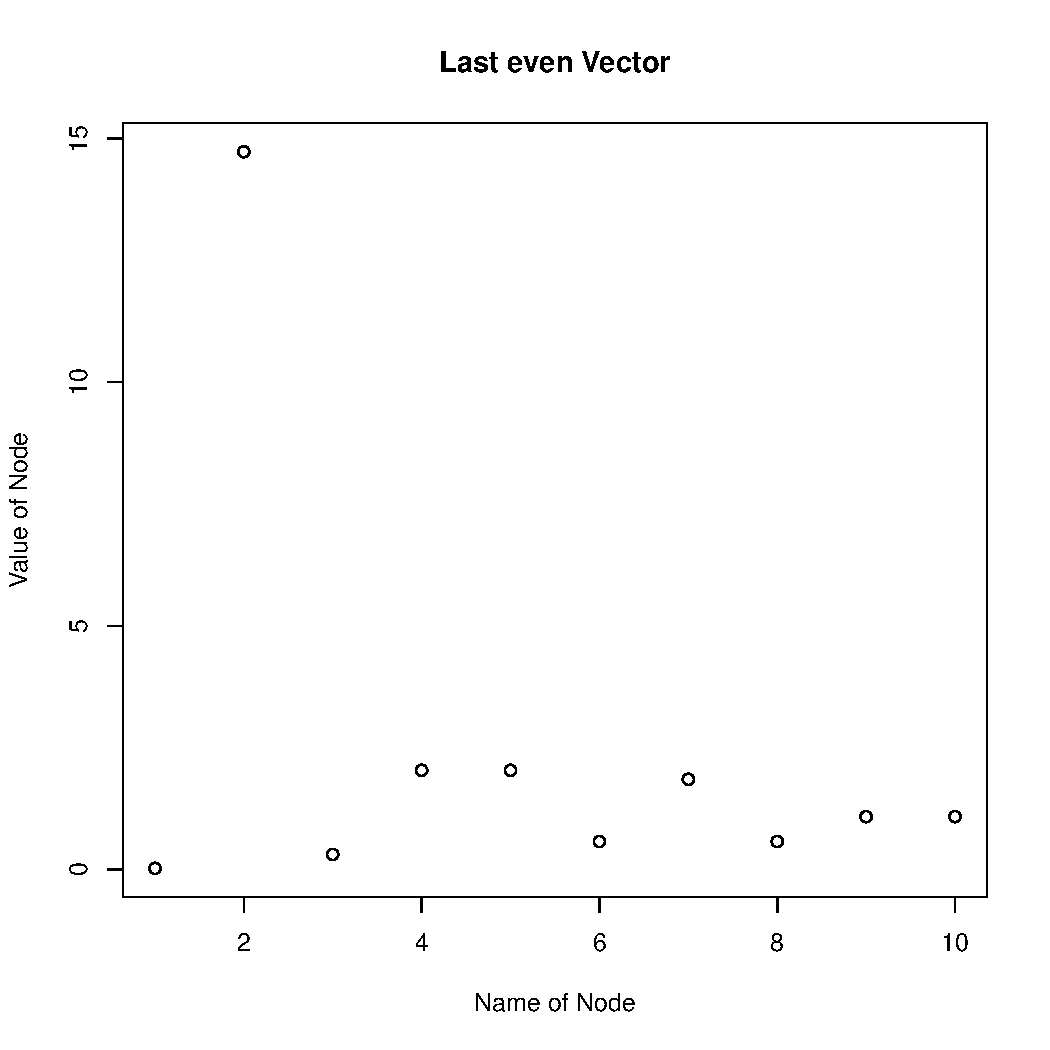
\includegraphics[width=\textwidth]{images/figures/evenResultVector.pdf}
        \caption{The centralities of each node in the last even vector of all iterations.}
        \label{fig:sub11}
    \end{subfigure}
    \begin{subfigure}[b]{.45\textwidth}
        \centering
        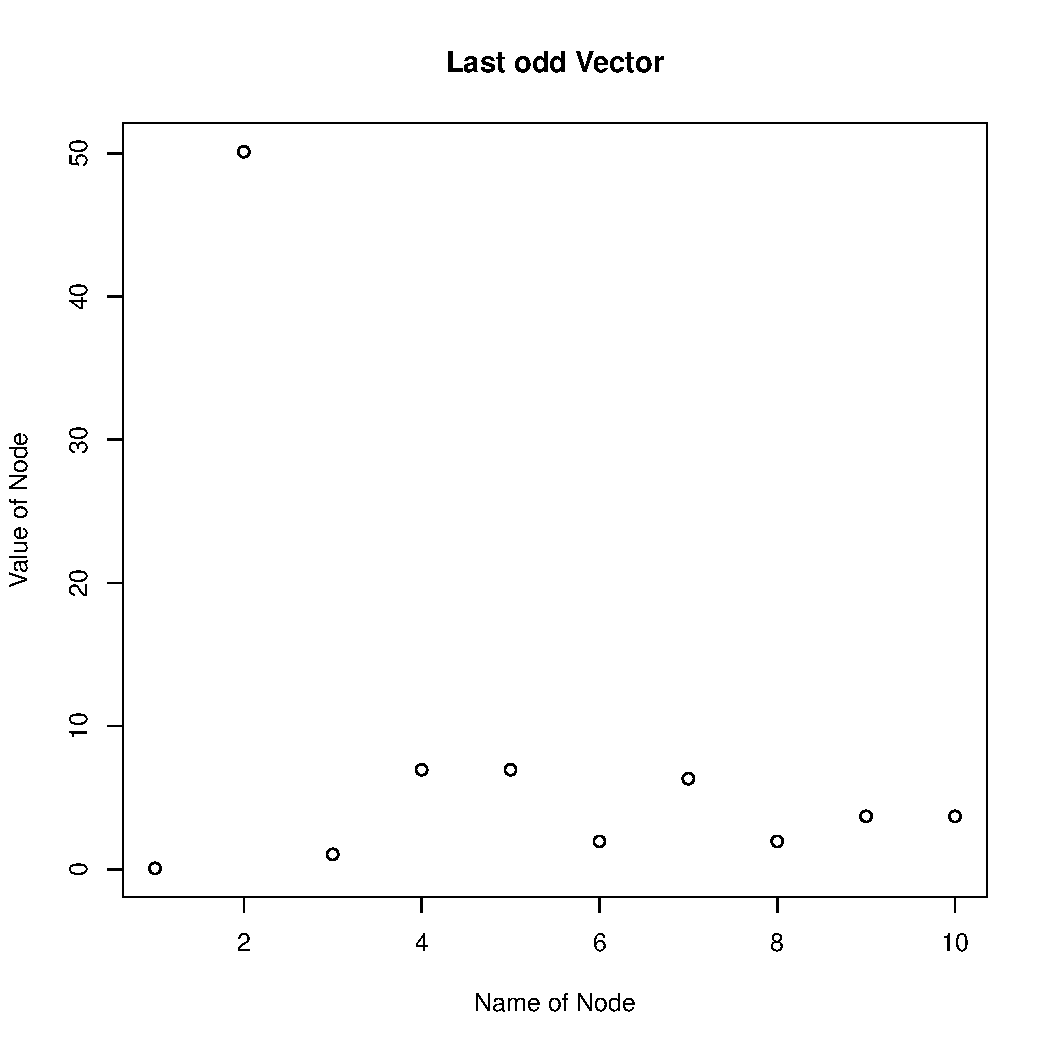
\includegraphics[width=\textwidth]{images/figures/oddResultVector.pdf}
        \caption{The centralities of each node in the last odd vector of all iterations.}
        \label{fig:sub12}
    \end{subfigure}%
    \label{fig:evenVSodd}
    \caption{The last even vector and the last odd vector paint the same picture and their values
    only differ by a multiplicative constant which can be seen nicely on the y axis.}
\end{figure}

Regarding the damage that the perturbation inflicts on the result, the impact becomes clear when
perturbing with $\alpha =0.1$ which will lead to faster convergence than $\alpha = 0.0001$ but
yield a false result with node $7$ as the most central one.

\begin{figure}[H]
    \centering
    \begin{subfigure}[b]{.45\textwidth}
        \centering
        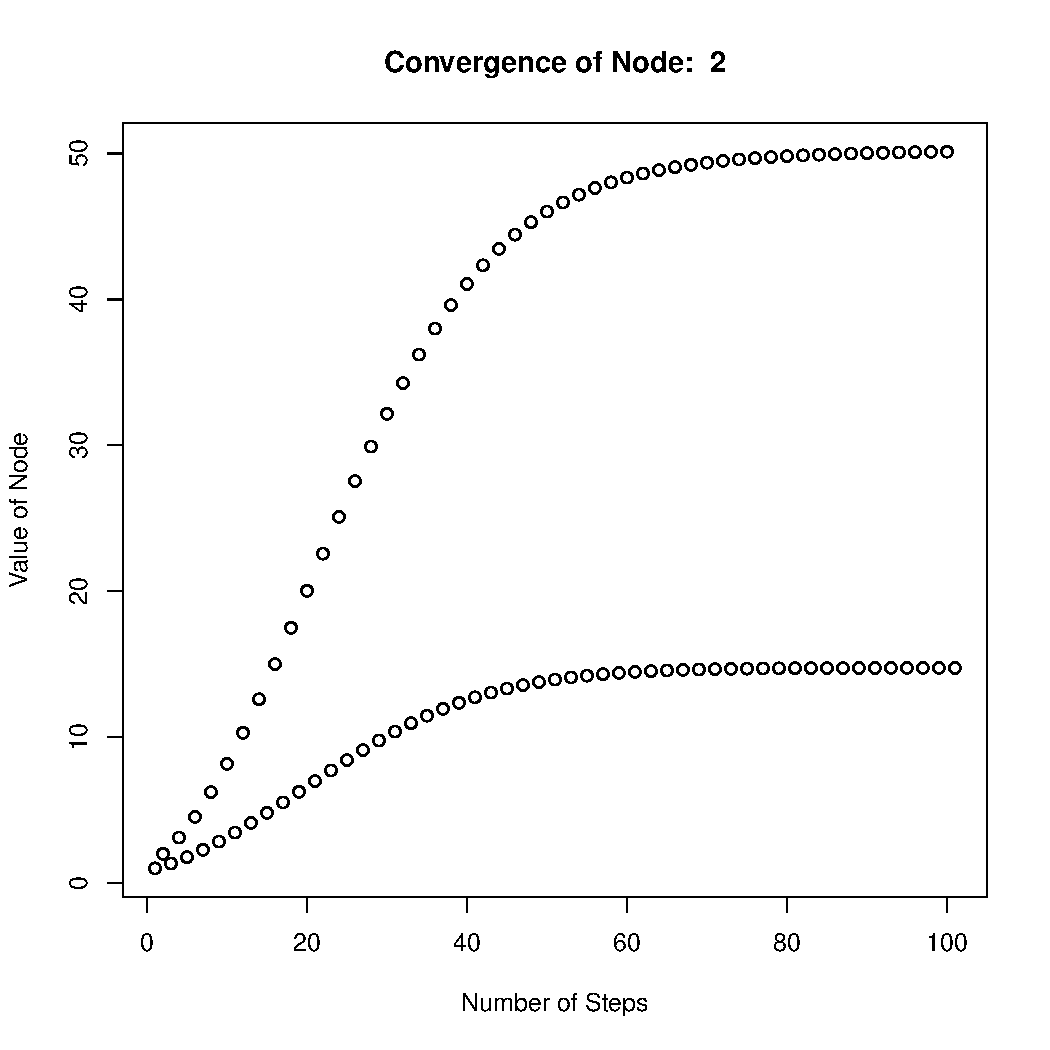
\includegraphics[width=\textwidth]{images/figures/convergence2.pdf}
        \caption{Convergence of $2$ with $\alpha = 0.0001$}
        \label{fig:sub22}
    \end{subfigure}
    \begin{subfigure}[b]{.45\textwidth}
        \centering
        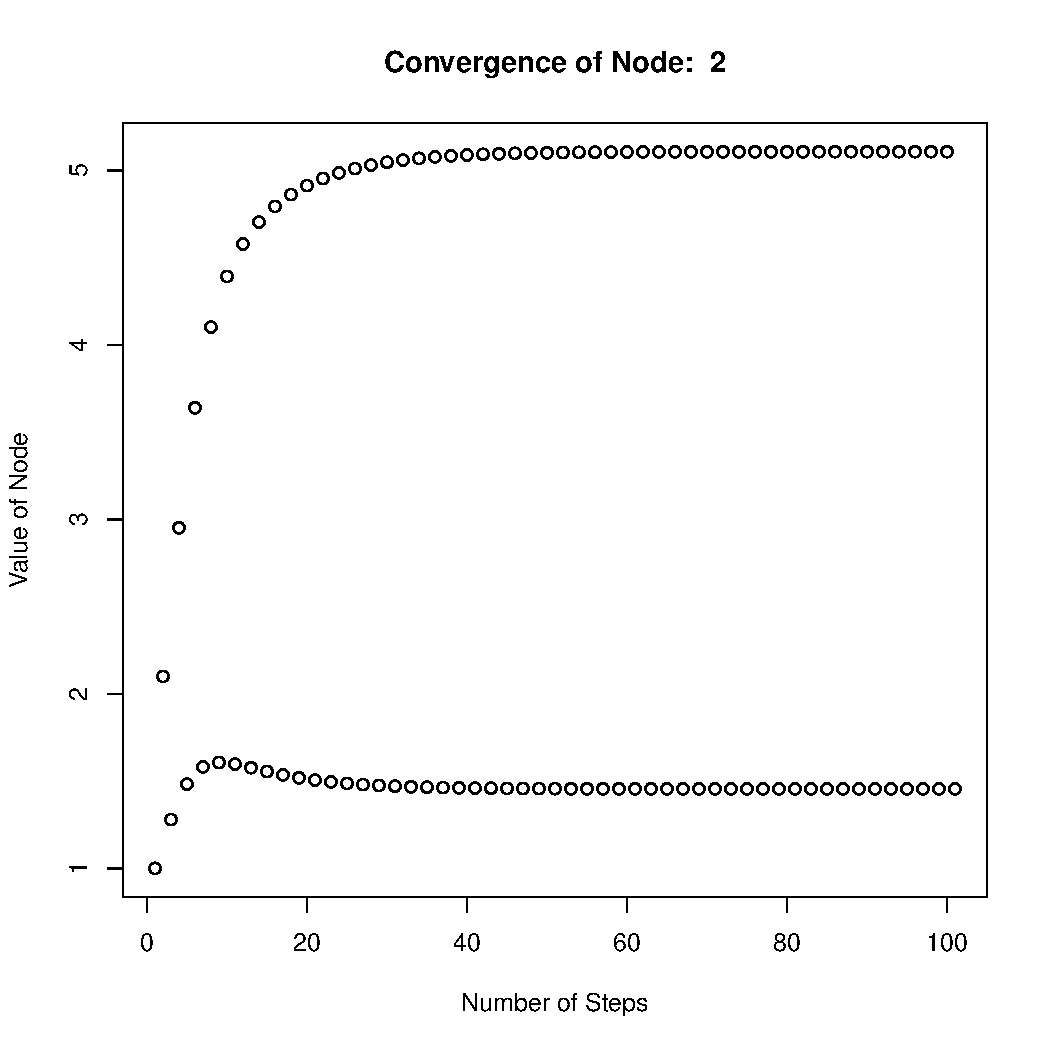
\includegraphics[width=\textwidth]{images/figures/convergence2badPerturbation.pdf}
        \caption{Convergence of $2$ with $\alpha = 0.1$}
        \label{fig:sub21}
    \end{subfigure}%
    \label{fig:impactOfPerturbation}
    \caption{The convergence for $\alpha = 0.1$ is faster but leads to a false result}
\end{figure}

%When a graph has no total support perturbation can be used to gain a solution. It is clear that
%perturbation impacts the convergence and the final result in some way. To see how large this
%impact is, a fully indecomposable matrix is taken and the Sinkhorn-Knopp method is applied. 
%The results are compared to the results of the Sinkhorn-Knopp method for the perturbed matrix. 